\documentclass{alk}

\usepackage{polski}
\usepackage{color}
\usepackage{tikz}
\usepackage{graphicx}
\usepackage{pbox}
\usepackage{amsmath}
\usepackage{mathtools}
\usepackage{algpseudocode}
\usepackage{amsthm}
\usepackage{caption}
\usepackage{subcaption}
\usepackage{minted}
\usepackage{epigraph}
\usepackage[nosingleletter]{impnattypo}
\usepackage{pictex}
\usepackage{rotating}
\usepackage{listings}
\usepackage{xcolor}
\usepackage{indentfirst}

\newcommand\TODO[1]{\textcolor{red}{TODO: #1}}

\author{Filip Stachura}
\title{Studium przypadku oraz indywidualne doświadczenia i wnioski związane z procesem coachingowym}
\kierunek{Coaching profesjonalny}

% miesiąc i rok:
\date{Czerwiec 2015}

\usepackage{tikz}
\usetikzlibrary{shapes,snakes}

\usepackage{hyperref}
\hypersetup{
    colorlinks,
    citecolor=black,
    filecolor=black,
    linkcolor=black,
    urlcolor=black
}

\usepackage{fontspec}
\setmainfont{Arial}

\usepackage[left=2.5cm,top=2.5cm,right=2.5cm,bottom=2.5cm,bindingoffset=0cm]{geometry}

\usepackage{setspace}
\onehalfspacing

\usepackage{amsthm}
\theoremstyle{definition}
\newtheorem{defn}{Definicja}

\usepackage{multirow}

% koniec definicji

\begin{document}

\maketitle

\tableofcontents

\chapter{Wstęp}

% Sgormułowanie własnej, indywidualnej definicji coachingu (uszczegółowioną i uzasadnioną). W jaki sposób osobiście
% rozumiem czym jest Coaching oraz kim /jestem/staję się w roli coacha?

Niniejsza praca poświęcona jest doświadczeniom zebranym przez autora w trakcie studiów podyplomowych na kierunku
\emph{Coaching profesjonalny}. Omawiane są również obserwacje i wnioski bazujące na tych doświadczeniach.
Praca została podzielona na trzy części. We wprowadzeniu została sformułowana indywidualna definicja coachingu,
która następnie została uzasadniona i porównana z definicją \emph{ICF}. Kolejna część, stanowiącą trzon pracy,
została podzielona na trzy podrozdziały, zawierające odpowiednio:
\begin{enumerate}
  \item Studium przypadku pracy z klientem, w którym dokładnie opisany jest jeden pełen proces coachingowy  , poprowadzony
      przez autora pracy w trakcie trwania studiów.
  \item Omówienie przez autora własnych doświadczenień związanych z coachingiem z perspektywy klienta. Autor bazuje na
      ćwiczeniach realizowanych z innymi studentami w ramach studiów i autocoachingu.
  \item Opinie na temat obszaru zastosowań procesu coachingowego oraz standardów etycznych.
\end{enumerate}
W ostatniej części pracy autor przedstawia swoją wizję dalszego rozwoju osobistego, ze szczególnym uwzględnieniem
obszaru umiejętności coachingowych. \\

\section{Indywidualna definicja coachingu}
Coaching jest forma wspomagania rozwoju, opartą o dialog pomiędzy coachem a klientem. Coach jest osobą odpowiedzialną za prowadzenie procesu.
Ze względu na swój niedyrektywny charakter, a również często niemierzalność efektów procesu coachingowego forma ta doczekała się
licznych definicji. Również w trakcie trwania studiów podyplomowych studenci mogli spotkać się z wieloma różnymi definicjami,
zależnie od wykładowcy prowadzącego zajęcia. Każda z tych definicji na swój sposób określa warunki tego procesu.
Jednocześnie w zdecydowanej większości przypadków definicje te nie są względem siebie sprzeczne, a raczej uzupełniają się
wzajemnie, tworząc razem pełniejszy obraz i budując intuicję słuchaczy o tym czym \emph{coaching} jest.

Pomimo wymienionych trudności stojących na przeszkodzie jednoznacznego zdefiniowania tej formy rozwoju istnieje grupa wymagań wspólnych dla
wszystkich definicji. Będą to na przykład te wymagania, które mówią o tym, że coaching to proces lub że jest współpracą pomiędzy
coachem a klientem. Indywidualna definicja autora tej pracy ma następującą treść:
\begin{defn}
  \emph{Coaching} jest dobrowolnym i niedyrektywnym, ograniczonym czasowo procesem partnerskiej współpracy,
  ukierunkowanym na rozwój klienta poprzez skupienie się na teraźniejszości i przyszłości.
  \label{definicja}
\end{defn}

W celu dokładnego wytłumaczenia przedstawionej definicji poszczególnie jej części zostały omówione niezależnie poniżej:

\subsection{Coaching jako proces dobrowolny}
Jednym z podstawowych założeń procesu coachingowego jest jego swobodna i nieobowiązkowa forma. Dotyczy to zarówno klienta, ale jest
również istotne z punktu widzenia coacha. Ponieważ obie strony mają świadomość swojego dobrowolnego uczestnictwa w spotkaniach pozwala to budować
zdrową relację opartą o niezależność wszystkich zaangażowanych osób.

\subsection{Coaching jako proces niedyrektywny}
Fundamentalnym założeniem jest powierzenie klientowi pełnej odpowiedzialności za podejmowane przez niego decyzje. W sposób naturany
warunek ten jest spełniony przez brak dyrektywnych rad i podpowiedzi od coacha. Ponieważ coach zadaje wyłącznie pytania klientowi,
a klient sam na podstawie pytań dochodzi do wniosków i rozwiązań, a ostatecznie swoich decyzji to naturalne jest branie odpowiedzialności
za te decyzję przez klienta. Zaakceptowanie tego wymagania powinno być warunkiem niezbędnym każdego procesu coachingowego.

Dodatkowym, bardzo ważnym czynnikiem jest również wysoka uwaga coacha na ustrzeganie się dyrektywności "\emph{nie wprost}". O takiej formie
dyrektywności mówi się wtedy, gdy coach przez zaniedbanie lub świadome działanie nakłania klienta do podjęcia pewnej decyzji bez uczciwego przeanalizowania
innych możliwości. \\

\subsection{Coaching jako proces ograniczony czasowo}
Zgodnie z tym stwierdzeniem coaching w pierwszej kolejności jest procesem. Ze Słownika Języka Polskiego można przytoczyć następującą definicję:
\begin{defn}
\emph{Proces} to przebieg następujących po sobie i powiązanych przyczynowo określonych zmian.
\end{defn}
Jednocześnie ten ciąg powiązanych ze sobą zmian ma być ograniczony czasowo. To założenie ma służyć dalszemu uniezależnieniu klienta
od coacha. Po zakończeniu procesu obie strony się rozstają, więc w najlepszym interesie klienta jest świadomie i jak najlepsze wykorzystanie
skończonej liczby sesji które może on odbyć.

\subsection{Coaching to partnerska współpraca}
Kolejną ważną koncepcją coachingu jest partnerski stosunek obu stron, w którym traktują one się wzajemnie w ten sam sposób. Dotyczy to zarówno
wymagań podstawowych, takich jak wzajemny szacunek czy zaangażowanie, ale również akceptacji i otwartości na inny punkt widzenia drugiej
osoby. Partnerska postawa powoduje, że w procesie coachingowym obie strony razem zmieżają do celu, ale jednocześnie obie zachowują
swoją niezależność. \\

Klasycznie współpraca ta jest budowana na fundamencie pytań, ale w swojej pracy coachowie wykorzystują również różnego rodzaju
narzędzia. Mają one na celu pobudzenie szukania kreatywnych rozwiązań przez klienta lub ułatwienie zaobserwowania
mu innego punktu widzenia danego zagadnienia.

\subsection{Coaching jest ukierunkowany na rozwój klienta}
Efektem procesu coachingowego powinna być trwała, pozytywna zmiana w życiu klienta. W przeciwieństwie do procesu terapeutycznego coaching
nie będzie miał na celu zdiagnozowania przyczyn zjawisk negatywnych, a skupii się na możliwych metodach ich przezwyciężenia. Jeszcze większej
uwagii wymaga ta część definicji kiedy w procesie uczestniczy również sponsor. Takim sponsorem może być na przykład pracodawca klienta.
To coach odpowiada za właściwe wytłumaczenie obowiązujących zasad klientowi i sponsorowi - w szczególności sponsor powinien mieć świadomość,
że w trakcie coachingu klient może podjąć decyzje niekorzystne z punktu widzenia sponsora.

\subsection{Coaching skupia się na teraźniejszości i przyszłości}
W celu ułatwienia klientowi przejęcia odpowiedzialności i ukierunkowania go na pozytywne rezultaty coaching koncentruje się na wydarzeniach
teraźniejszych i przyszłych. Coaching wychodzi z założenia, że na wydarzenia przeszłe nie ma się wpływu i powinno się je w pełni zaakceptować.
Oczywiście wyciąganie wniosków z przeszłych wydarzeń może okazać się cenną lekcją na przyszłość, ale nadmierne
rozpamiętywanie przeszłości będzie prawdopodobnie blokować klienta zamiast posuwać go naprzód.

\section{Porównanie z innymi formami rozwoju osobistego}
Przy definiowaniu \emph{coachingu} wartościowe jest umiejscowienie tego pojęcia względem innych form rozwoju osobistego.
W tabeli \ref{table:kategorie} został skategoryzowane najbardziej popularne formy rozwoju ze względu na swój dyrektywny
i niedyrektywny charakter oraz czas trwania procesu.

\begin{table}[!ht]
  \centering
  \caption*{Formy rozwoju osobistego}
  \def\arraystretch{1.5}
  \begin{tabular}{c|c|c|}
    \cline{2-3}
    & \emph{Dyrektywne} & \emph{Niedyrektywne} \\ \cline{1-3}
    \multicolumn{1}{|c|}{\multirow{3}{*}{\emph{Ograniczone czasowo}} } & Mentoring & Coaching \\
    \multicolumn{1}{|c|}{} & Nauka & Counseling \\
    \multicolumn{1}{|c|}{} & & Doradztwo \\ \cline{1-3}
    \multicolumn{1}{|c|}{\multirow{1}{*}{\emph{Nieograniczone czasowo}} } & Trening & Terapia \\ \cline{1-3}
  \end{tabular}
  \caption{Formy rozwoju osobistego skategoryzowane ze względu na czas trwania procesu oraz swój dyrektywny lub niedyrektywny charakter.}
  \label{table:kategorie}
\end{table}

\subsection{Czym różni się coaching od mentoringu?}

O ile w coachingu każdą decyzje lub wniosek klient podejmuje sam, to w mentoringu otrzymuje on sprawdzone, gotowe rozwiązania od mentora.
Mentoring często wykorzystywany jest w organizacjach, gdzie doświadczony pracownik jest mentorem dla osoby zaczynającej pracę na danym stanowisku.

Elementem procesu coachingowego będzie upewnienie się, że klient faktycznie chce zrealizować swój cel i że akceptuje jego konsekwencje.
Mentoring nie ma takiego holistycznego charakteru - skupia się na danym zagadnieniu i dostarcza wiedzę i umiejętności dla klienta.
Wspólnym mianownikiem jest ograniczenie czasowe nałożone na oba procesy.

\subsection{Czym różni się coaching od terapii?}
Główne różnice są dwie: \\
- Terapia nie musi być ograniczona czasowo i może mieć długotrwały charakter. \\
- W terapii klient nie przejmuje odpowiedzialności za proces - w procesie terapeutycznym terapeuta prowadzi klienta.

Podobieństwo między coachingiem, a terapią polega na ich niedyrektywnym charakterze. Terapeuta nie daje klientowi gotowych rozwiązań, które mogłyby
zostać bezpośrednio zastosowane w przypadku tej osoby.

\subsection{Czym różni się coaching od doradztwa?}
Doradztwo ma na celu dostarczenie klientowi wiedzy na temat jego obecnej sytuacji i możliwości które przed nim stoją. Doradca jako ekspert dokonuje
dokładnej analizy informacji otrzymanych od klienta i bazując na swoim doświadczeniu przedstawia klientowi propozycje, które uważa za najskuteczniejsze.
Z tego powodu doradca przejmuje część odpowiedzialności za wybory swojego klienta. Podobnie jak coaching proces doradczy jest ograniczony czasowo.

\subsection{Czym różni się coaching od nauki?}

Klasyczny proces uczenia polega na przekazaniu określonego zakresu wiedzy w ramach realizowanego programu, w określonym czasie. Uczeń ma za zadanie
przyswajać wiedzę teoretyczną oraz realizować ćwiczenia wyznaczane przez nauczyciela. Zazwyczaj pod koniec procesu nauki uczeń przystępuje do egzaminu
weryfikującego poziom jego wiedzy i umiejętności w danej dziedzinie. W porównaniu do coachingu w procesie nauki określone są bardzo sztywne wzorce
oraz mierzalne cele.

\subsection{Czym różni się coaching od counselingu?}

Podstawową różnicą pomiędzy coachingiem a counselingiem leży w postawionym celu. O ile coaching jest przede wszystkim nastawiony na realizację celów
klienta, to counseling ma za zadanie pomóc w rozwiązaniu pojawiających się problemów czy trudności. Jest on doradzany na przykład osobom zmagającym się
z wypaleniem zawodowym, problemami emocjonalnym lub w relacjach. Z tego powodu counseling pod niektórymi względami przypomina proces terapeutyczny.
Jednocześnie podobnie do coachingu w tym wypadku współpraca jest ograniczona czasowa.

\subsection{Czym różni się coaching od treningu?}

Trening jest długotrwałym procesem, w którym trener korzystając z swojej wiedzy i doświadczenia ustala realizowany plan treningowy. Poprzez wytrwały
trening oraz mierzenie osiąganych wyników wypracowywane są coraz lepsze rezultaty. Trening podobnie do mentoringu jest nastawiony na uzyskanie
jak najlepszych rezultatów, ale ma długotrwały charakter, w którym systematyczność i wytrwałość mają największe znaczenie.

\section{Porównanie z definicją ICF}
Podsumowanie tego rozdziału stanowi porównanie z definicją jednej z największych organizacji zrzeszających pasjonatów coachingu:
International Coach Federation (ICF) \cite{deficf}.

\begin{defn}
ICF definiuje coaching jako partnerstwo z klientem w prowokującym myślenie, kreatywnym procesie, który inspiruje ich do maksymalizacji ich
osobistego i zawodowego potencjału, co jest niezwykle istotne w dzisiejszym niepewnym i złożonym środowisku. (tłum. własne
\footnote{ICF defines coaching as partnering with clients in a thought-provoking and creative process that inspires them to maximize
their personal and professional potential, which is particularly important in today's uncertain and complex environment.})
\end{defn}

Bardzo czytelne podobieństwa pomiędzy tymi dwiema definicjami to bardzo wyraźne podkreślanie partnerskiego charakteru relacji klient-coach
oraz ukierunkowanie procesu na rozwój klienta. W definicji przedstawionej w tej pracy coach otrzymuje większą swobodę przy kreaowaniu procesu, bez
potrzeby podkreślanie jego kreatywnej i prowokatywnej formy. Z drugiej strony zgodnie z tą definicją nacisk położony jest na skupienie się na
teraźniejszość i przyszłość, co nie jest dosłownie podkreślone w definicji ICF.

Istotną różnicą pomiędzy definicjami jest brak wymagania określenia ograniczonych ram czasowych dla procesu coachingowego. Również w innych materiałach
udostępnianych przez ICF dopuszczane są procesy trwające więcej niż wiele miesięcy, a sama istota określenia ram czasowych nie jest wyraźnie w tych materiałach
podkreślona. Zdaniem autora jest to bardzo istotne wymaganie i w sposób wartościowy wzbogaca ono definicję ICF.

Ostatnią z opisanych różnic jest opis dzisiejszego środowiska, mającego wpływ na istotność coachingu w dzisiejszym świecie. Zdaniem autora jest to część
nie przekazująca dodatkowych informacji czym coaching jest i przez to zbędna. Merytoryczne dyskusja na temat tego czy coaching jest w dzisiejszych czasach
niż w przeszłości mogłaby być ciekawym eksperymentem naukowym, ale nie ma ona wpływu na to czym coaching jest.


\chapter{Część zasadnicza}

\section{Studium przypadku}
% Opis jednego procesu coachingowego z zachowaniem poufności poprzez zapewnienie anonimowości osoby coachowanej (min. 5 sesji z jednym klientem.

W tej sekcji został opisany proces coachingowy realizowany w trakcie trwania studiów podyplomowych, prowadzony przez autora pracy. Klientką była
młoda kobieta na wczesnym etapie swojej kariery zawodowej. Jest to osoba rzeczowa, o wysokiej motywacji i nastawieniu na realizację celu.

Krótki czas przed rozpoczęciem procesu coachingowego klientka otrzymała awans, co sprawiło,
że stanęła przed zupełnie nowymi wyzwaniami i z niektórymi współpracownikami musiała zmienić dotychczasową relację. W niektórych przypadkach oznaczało
to, że stała się przełożoną swoich dotychczasowych kolegów i koleżanek z pracy. Jej nowe obowiązki obejmowały między innymi definiowanie celów pośrednich,
harmonogramu projektów, dawanie informacji zwrotnej pracownikom, dbanie o poziom motywacji i atmosfery w zespole złożonym ze specjalistów. Warto podkreślić,
że klientka wcześniej sama obejmowała stanowisko eksperckie, na którym tego typu działania nie wchodziły w zakres jej obowiązków.

\subsection{Początkowe wyzwania i cele klienta}
% punkt wyjścia - wyzwania i cele klienta

Pierwsza odbyta sesja miała na celu potwierdzenie chęci obu stron do rozpoczęcia pracy coachingowej, następnie ustalenie kontraktu, aby potem wybrać obszar
i cele do realizacji w trakcie trwania okresu coachingu. Pierwszym wyzwaniem okazał się element edukacyjny. Pomimo, że klientka jest osobą dobrze
wykształconą, oczytaną i posiadającą wszechstronną wiedzę, jej wiedza na temat coachingu była na bardzo niskim poziomie. Coachowana\footnote{Proponowany
tłumaczenie angielskiego sformułowania \emph{coachee}, zgodnie z \url{http://sjp.pwn.pl/poradnia/haslo/coachee-mentee;10085.html}} wiedziała, że coaching
jest modną i zyskującą ciągle na popularności formą rozwoju osobistego. Na tych informacjach jej wiedza na temat coachingu się kończyła. Jednocześnie
klientka żywiła pewne obawy dotyczące samego procesu. Najważniejsza z nich dotyczyła zachowania niezależności w doborze tematów coachingu oraz prywatności
osobistej.

Autor pracy jako coach wyjaśnił klientce najważniejsze założenia coachingu oraz umiejscowił go względem innych form rozwoju osobistego, podobnie jak miało to miejsce
w rozdziale pierwszym. Klientka po wysłuchaniu i zrozumieniu tych informacji wyraziła gotowość do wejścia w proces coachingowy, decyzja była podjęta
z dużą gotowością na poznanie czegoś nowego oraz motywacją do wykorzystania jak najlepiej pojawiającej się okazji rozwoju. Po tej deklaracji coach również
był gotowy do rozpoczęcia pracy, mając na uwadze posiadaną już przez klientkę wiedzę i jej wysoką motywację. W związku z tym obie strony przystąpiły
do ustalenia wspólnie kontraktu coachingowego.

Kontrakt zapewniał obu stronom pełną prywatność informacji omawianych w trakcie pracy coachingowej.
Coachowana została poinformowana o późniejszym, anonimowym opisaniu procesu na rzecz niniejszej pracy dyplomowej.
Klientka otrzymała zapewnienie posiadania pełnej kontroli nad zakresem tematów
poruszanych na sesjach. Jest to całkowicie naturalne, że klient decyduje o poruszanych tematach. Można więc zastanawiać się, czy podkreślanie tego explicite
w kontrakcie jest istotne. W tym wypadku coach stwierdził, że ponieważ jest to obszar wątpliwy dla klientki to wyraźne podkreślenie tego ustalenia
będzie dla niej pomocne. Coach i coachowana umówili się również na dopilnowanie regularności swoich spotkań oraz dbanie o wysoki poziom energii na sesjach.


Ostatnim elementem pierwszej sesji było wyznaczenie tematyki i celów dla całego lub części procesu. Klientka sama przychodząc na sesję nie miała określonych
konkretnych zamiarów i celów. Coach wykorzystał narzędzie \emph{,,Koło życia''}, co bardzo szybko pozwoliło stwierdzić coachowanej, że chce zająć się obszarem
rozwoju zawodowego. Decydujący wpływ na tę decyzję miał opisany wcześniej awans i nowe wyzwania z nim związane.

Po skutecznym określeniu obszaru, którego miał dotyczyć proces coachingowy, przystąpiono do ustalenia celów i efektów tego procesu. Po krótkiej przerwie
coach wykonał wraz z klientką około 20-minutowa sesję dodatkową, opartą o model \emph{GROW}. Wykorzystując ten model w kolejnych krokach omawia się:
\begin{enumerate}
  \item Cel (ang. \emph{goal}).
  \item Stan obecny - rzeczywistość (ang. \emph{reality}).
  \item Przeszkody i możliwości (ang. \emph{obstacles / options}).
  \item Wolę (ang. \emph{will}).
\end{enumerate}

W oparciu o ten model klientka zdefiniowała swoją obecną sytuację zawodową i zaobserwowała możliwości, jakie stwarza jej obecna sytuacja. Mając świadomość
tego, z czego może wybrać i ile ma zasobów podjęła decyzję o skupieniu się na trzech konkretnych umiejętnościach:
\begin{itemize}
  \item Umiejętności organizacji pracy członków koordynowanego zespołu.
  \item Skutecznym stawianiu wymagań.
  \item Umiejętności właściwego i skutecznego przekazywania informacji zwrotnej.
\end{itemize}

Dla każdej z tych umiejętności klientka chciała określić mierzalne metody oceny, mające służyć sprawdzeniu stopnia poprawy w danym zakresie. Nie było
to zadanie łatwe dla klientki, ponieważ wszystkie trzy umiejętności dotyczą tak zwanych kompetencji ,,miękkich''. Ostatecznie dla pierwszej umiejętności
klientka postanowiła wprowadzić w zespole system mierzenia opóźnień prac względem wyznaczonych wspólnie celów, a dla drugiej liczenie liczby przypadków
nieporozumień dotyczących wyznaczonych zadań. Największe problemy sprawiła ostatnia z umiejętności. W tym wypadku klientka postanowiła zapisywać własne
odczucia dotyczące przeprowadzanych rozmów i śledzić te notatki. Tego typu decyzja wynikła z oceny klientki, że w danym momencie jest w stanie z dużą
dozą pewności ocenić czy odbyta rozmowa była skuteczna. Jednocześnie potrafi ona sprawdzić czy zachowała inne stawiane przez nią wymagania (np. dbanie o atmosferę w zespole).
Jej obawy dotyczyły braku możliwości obserwowania procesu prac nad tą umiejętnością z perspektywy czasu.

\subsection{Proces coachingowy}
%) proces - nad czym pracowano na jakich poziomach zachodziły zmiany co stanowiło szególne wyzwanie w pracy akurat z tym klientem?

Z perspektywy coacha zrealizowany proces coachingowy można podzielić na dwa etapy. W trakcie trwania pierwszego etapu w ramach sesji klientka
analizowała swoją obecną sytuację w życiu oraz rozwiązywała różnego rodzaju bieżące, pilne dla niej zagadnienia, w oparciu o metody coachingowe.
W trakcie trwania tego etapu można było zaobserwować wzrost samoświadomości dotyczącej własnych umiejętności, potrzeb, a także budowanie i przyswajanie
strategii skutecznego działania. Drugi etap był ukierunkowany na przyszłość i skupił się na określeniu długofalowych potrzeb klientki i budowie rocznego
planu działania mającego być realizowanym samodzielnie po zakończeniu współpracy z coachem.

Podstawowym narzędziem pojawiającym się często w pierwszym etapie był model \emph{GROW}. Został on zastosowany kilkukrotnie do mniejszych zadań
którymi klientka chciała zająć się w ramach sesji. Standardowy schemat wyglądał w tym wypadku tak, że klientka przychodziła na sesję coachingową
z ustalonym zadaniem, na które chciała poświęcić czas w ramach coachingu. Ciekawą z punktu widzenia coacha obserwacją było wytwarzanie się, wraz z upływem
czasu, u klientki naturalnej strategii planowania działań. Z każdym kolejnym zastosowaniem modelu \emph{GROW} klientka szybciej potrafiła zastosować
go w pojawiających się sytuacjach, ale co ważniejsze - w sposób intuicyjny sama stosowała go indywidualnie poza sesjami coachingowymi. Można również liczyć,
że wzorce te zostały również przeniesione na inne obszary życia, niekoniecznie związane ze sferą zawodową. Ten wniosek wymagałby jednak dodatkowych
informacji ponieważ w ramach sesji poruszane były jedynie tematy zawodowe.

Bardzo ważnym, zdaniem coacha, tematem poruszonym w ramach jednej z pierwszych sesji był dylemat klientki dotyczący jej nowej roli.
Z jednej strony klientka wyrażała dużą mobilizację i chęć do realizacji w nowej roli. Z drugiej strony równocześnie wyrażała chęć realizacji
eksperckich zadań, co dawało jej w przeszłości bardzo dużą satysfakcję i pewność, że powierzone jej zadania są wykonywane na odpowiednim poziomie.
Wejście w rolę lidera sprawiło, że główny wkład w realizację celów nie był wymierny, a jedynie pośredni - to budziło w klientce obawę.
Jednocześnie klientka wyraziła niepokój, że próba realizowania się w obu zadaniach może ją doprowadzić do porażki na obydwóch obszarach.

Najważniejszym, zdaniem coacha, ćwiczeniem dotyczącym tego dylematu był \emph{,,Diament kartezjański''}.
Coachowana zmierzyła się z dylematem poprzez odpowiedź na cztery pytania, gdzie za każdym razem zastanawiała się z czym związana jest zmiana
roli eksperta/inżyniera na rolę lidera:
\begin{enumerate}
\item Co się stanie, jeśli to zrobisz?
\item Co się stanie, jeśli tego nie zrobisz?
\item Co się nie stanie, jeśli to zrobisz?
\item Co się nie stanie, jeśli tego nie zrobisz?
\end{enumerate}
Dzięki wnioskom z tego ćwiczenia klientka podjęła decyzję o pozostaniu w nowej roli. Kluczowym czynnikiem było tutaj stwierdzenie, że posiada
ona predyspozycje do nowej roli i długofalowo będzie w niej bardziej skuteczna niż w roli inżyniera. Praca z tym dylematem była dla coacha
największym wyzwaniem w trakcie całego procesu coachingowego. Poruszony dylemat dotyczy obszarów wartości i tożsamości klienta. Interpretacja
decyzji klientki może być taka, że ważnym elementem jej życiowej misji jest tworzenie. Klientka oceniła więc, w której z ról będzie mogła skuteczniej
realizować swoją misję i na tej podstawie dokonała wyboru.

Z perspektywy coacha, autor pracy uważa, ze dylemat ten został na pewien czas załagodzony. Jako coach widzi tutaj własną możliwość wzrostu poprzez
skuteczniejszą możliwość pomocy klientowi w tak trudnych wyborach. Dodatkowo jako coach, autor jest zadowolony, że decyzję i odpowiedzialność za nią
ponosi w pełni klient i w przyszłości zapewne powróci do tego dylematu, z większą wiedzą i doświadczeniem.

Kolejnym i ostatnim już ćwiczeniem omówionym w ramach tej pracy i dotyczącym pierwszego etapu jest narzędzie \emph{Figure it out} zaproponowane
w trakcie trwania studiów przez Artura Rzepackiego. W ramach tego ćwiczenia klient definiuje różnego rodzaju realizowane zadania w swojej
organizacji poprzez symbole, takie jak trójkąty, kwadraty, koła itd.. Następnie dla występujących w organizacji stanowisk przypisuje pewien
zbiór symboli, stałej wielkości, mający określić idealne zdaniem klienta wykorzystanie zasobów czasowych do realizacji obowiązków danej osoby.
Przykładowe przyporządkowanie symboli do stanowisk przedstawione jest na rysunku \ref{table:figureitout}.

\begin{table}[!ht]
  \centering
  \caption*{Narzędzie coachingowe: ang. \emph{Figure it out} }
  \def\arraystretch{2}%  1 is the default, change whatever you need
  \begin{tabular}{|l|c|c|c|c|c|c|c|}
  \hline
  Zarząd & 
\includegraphics{img/s4} & 
\includegraphics{img/s4} & 
\includegraphics{img/s4}  & 
\includegraphics{img/s3} & 
\includegraphics{img/s2} & 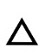
\includegraphics{img/s1} & 
\includegraphics{img/s4} \\ \hline
  Dyrektor & 
\includegraphics{img/s3} & 
\includegraphics{img/s3} & 
\includegraphics{img/s3} & 
\includegraphics{img/s2} & 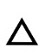
\includegraphics{img/s1} & 
\includegraphics{img/s3} & 
\includegraphics{img/s4} \\ \hline
  Kierownik & 
\includegraphics{img/s2} & 
\includegraphics{img/s2} & 
\includegraphics{img/s2} & 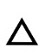
\includegraphics{img/s1} & 
\includegraphics{img/s2} & 
\includegraphics{img/s2} & 
\includegraphics{img/s3}\\ \hline
  Specjalista & 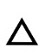
\includegraphics{img/s1} & 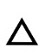
\includegraphics{img/s1} & 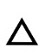
\includegraphics{img/s1} & 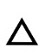
\includegraphics{img/s1} & 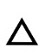
\includegraphics{img/s1} & 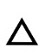
\includegraphics{img/s1} & 
\includegraphics{img/s2}\\ \hline
  \end{tabular}
  \caption{Przykładowe przyporządkowanie symboli realizowanych zadań do stanowisk w organizacji.}
  \label{table:figureitout}
\end{table}

Kolejnym krokiem przy realizacji tego ćwiczenia jest określenie zbioru symboli tej samej wielkości dla jego obecnej sytuacji.
Przy omawianym w tym rozdziale procesie coachingowym została również omówiona sytuacja członków zespołu prowadzonego przez klientkę.
Efektem ćwiczenia było przede wszystkim uświadomienie sobie przez klientkę, że nadal realizuje za dużo zadań związanych ze starą rolą ekspercką.
Drugim ciekawym wnioskiem była obserwacja, że w nowej roli jest również dla niej ważne uważne przyglądanie się i częściowa realizacja zadań
osób będących na jeszcze wyższych stanowiskach. \\

Drugi etap procesu był zauważalnie krótszy od pierwszego. Podczas jego trwania klientka czuła się już znacznie swobodniej w nowej roli, ale również współpraca
z coachem stała się czymś bardziej naturalnym. Na tym etapie główny nacisk został położony na dalszy rozwój po zakończeniu procesu coachingowego
oraz ustalenie planu działania na najbliższy rok.

Do zaadresowania potrzeby dalszego rozwoju osobistego zostało wykorzystane narzędzie wprowadzone na zajęciach z Panem Maciejem Bennewiczem. W ramach tego
ćwiczenia klient analizuje cztery możliwe metody rozwoju: uczenie się, coaching, mentoring i doradztwo. Dla każdej z tych metod zastanawia się,
co ważnego i cennego mógłby lub powinien zrobić z jej wykorzystaniem. Co może być interesujące, w ramach tego ćwiczenia coach otrzymał od klientki
niebezpośrednią informację zwrotną na temat korzyści wynikających jej zdaniem z zaangażowania się w proces coachingowy. Zostaną one omówione w
następnej sekcji.

W celu ustalenia planu działania na kolejny rok użyte zostały karty Dixit
\footnote{Gra karciana pobudzająca wyobraźnie - \url{https://pl.wikipedia.org/wiki/Dixit}}. Narzędzie to zostało zaprezentowane na zajęciach
prowadzonych przez Panię Katarzynę Ramirez-Cyzio. Klient w trakcie tego ćwiczenia wybiera kartę, która reprezentuje dla niego sytuację po roku czasu,
a następnie układa pełny przebieg zdarzeń przy pomocy wybranych przez niego kart. Ćwiczenie można urozmaicać pytając na przykład o osoby, które powinny
pojawić się na drodze klienta. W dowolnym momencie klient poprawia układ kart na osi czasu, ale pod koniec ćwiczenia powinien zaakceptować finalny układ.

Na ostatniej sesji dzięki wykorzystaniu tego narzędzia został zbudowany plan działania na przyszłość. Ćwiczenie to pomogło również zakończyć
proces coachingowy w zrównoważony sposób i wycofać coacha z życia klientki.

\subsection{Uzyskane efekty i dalsze cele}
%) efekty - stan docelowoy - co zrealizowano, jakie dalsze postępowanie byłoby wskazane?

Z perspektywy całego procesu coachingowego określenie uzyskanych efektów i podsumowanie zaistniałych zmian zazwyczaj nie jest zadaniem łatwym.
Wynika to z faktu, że wiele z nich zachodzi w sposób długotrwały i niemierzalny. Przykładami takich zmian mogą być zmiany przekonań klienta lub
rozpoczynające proces rozwoju na jakimś polu - na przykład budowanie autorytetu wśród zespołu.

W celu zbudowania takiego podsumowania ważne staje się obserwowanie również zmian w postrzeganiu klienta i jego decyzji, a nie tylko jego zachowań
czy uzyskiwanych mierzalnych efektów. Ważnym elementem przy budowie tego typu podsumowania jest również uzyskanie opinii samego klienta na temat
przeprowadzonego procesu. W zależności czy klient postrzega poświęcony czas jako wartościowy lub bezwartościowy efektywność procesu będzie,
z bardzo dużym prawdopodobieństwem, różnić się diametralnie.

Do najbardziej istotnych efektów procesu należały:
\begin{itemize}
  \item Klientka nauczyła się samodzielnie i intuicyjnie stosować model \emph{GROW} do realizacji swoich celów zawodowych.
  \item W sposób regularny realizowane były cele wypracowywane w ramach sesji coachingowej. Dotyczyły one głównie wyznaczonych na
      pierwszej sesji obszarów: organizacji pracy, stawianie wymagań i dawania informacji zwrotnej.
  \item Jak klientka sama stwierdziła w trakcie jednego z ćwiczeń, największą korzyścią jej zdaniem było regularne poświęcanie czasu na zastanowienie
      się nad pojawiającymi się w jej życiu zagadnieniami. Zauważyła, że przy wysokim tempie życia wiele istotnych decyzji mogłoby zostać zmarginalizowanych,
      a dzięki spotkaniom w ramach sesji coachingowych poświęcała im właściwą uwagę. Prawdopodobnie cenne będzie tutaj dokładne przytoczenie słów klientki:
      \begin{quote}
      \centering
      \emph{,,Sama też bym to potrafiła, ale dzięki temu naprawdę to robię.''}
      \end{quote}
      Nawiązując do rozdziału pierwszego niniejszej pracy, w którym rozważana jest definicja coachingu, można zauważyć, że to jedno zdanie również
      może służyć za wymowną definicję procesu coachingowego.
\end{itemize}

Pod koniec procesu zostały wyznaczone następujące przyszłe cele:
\begin{itemize}
  \item Klientka określiła kolejne cele związane z rozwojem osobistym: pierwszym z nich jest znalezienie mentora, a drugi to pozyskiwanie dalszej wiedzy
      w ramach szkoleń i samodzielnej nauki.
  \item Ustalony został przez klientkę roczny plan rozwoju zawodowego.
\end{itemize}

\subsection{Retrospekcja z punktu widzenia coacha}
% feedback - czego, jako coach w tym procesie dowiedziałem się o sobie/ swoich kompetencjach / postawie coacha
%          - jakie dlasze zadania rozwojowe w roli coacha przede mna?

Dla autora pracy był to pierwszy w pełni przeprowadzony proces coachingowy. To pierwsze doświadczenie doprowadziło do wielu cennych wniosków.

Pierwsza cenna wiedza płynie z samego początku procesu - pierwszego spotkania z klientem. Bardzo ważne jest dobre przygotowanie się do tego spotkania,
ponieważ wcześniej coach nie ma żadnych informacji na temat stanu wiedzy swojego klienta. Coach powinien bez trudności wyjaśnić nie tylko czym jest coaching,
ale również czym charakteryzują się inne formy rozwoju i jakie są podobieństwa i różnice między nimi. Jest to szczególnie istotne w przypadku
klienta, dla którego są to pierwsze doświadczenia związane z coachingiem i może mieć złe wyobrażenie o tym jak wygląda taki proces.

Drugim wnioskiem, który może zostać wyciągnięty z tych doświadczeń jest skuteczność procesu coachingowego. W trakcie trwania procesu coach mógł zaobserwować
zmiany zachodzące w życiu klienta i usłyszeć jego zdanie na temat skuteczności wprowadzanych zmian. Dodatkowo coach zauważył, że zachodzące zmiany
mają głębszy charakter i są skuteczniejsze niż w przypadku pojedynczych sesji lub w przypadku zaangażowania emocjonalnego coacha w relację z osobą
coachowaną. Dzięki temu doświadczeniu coach nauczył się, że przeprowadzanie ćwiczeń na przykład z osobami bliskimi lub przyjaciółmi może być nieskuteczne
i jest zadaniem dużo trudniejszym niż ćwiczenie z osobami obcymi - względem których nie jest się zaangażowanym emocjonalnie.

Ostatnim wnioskiem jest podobieństwo roli coacha do roli mentora. Na początku studiów podyplomowych autor pracy miał poczucie, że są to dwie bardzo
dalekie od siebie formy rozwoju. Wraz ze zbieranym doświadczeniem zauważył jednak, że coach, podobnie jak mentor, również w pewnym sensie uczy swojego klienta.
W tym wypadku jednak nauka nie polega na przekazaniu konkretnej wiedzy, a metod analizy sytuacji z wielu perspektyw, kreatywnego podejścia lub
strategii myślenia skutecznych przy budowaniu strategii realizacji celów (takich jak \emph{GROW}). Po zakończeniu procesu coachingowego klient wyposażony
w te umiejętności jest gotowy do samodzielnego ich wykorzystywania w przyszłości.


\section{Własne doświadczenie coachingu}

% Na podstawie sesji kiedy bylem osoba coachowana i cwiczen, ktore byly zwiazane z autocoachingiem.
% Jakie korzysci proces coachingowy przyniosl mi, na jakich poziomach piramidy Diltsa obserwuje zachodzace zmiany?
% Co ma dla mnie najwieksze znaczenie/ jest dla mnie najwieksza wartoscia z zaangazowania sie we wlasny proces coachingowy?

W tym rozdziale autor pracy omówi korzyści i zmiany pojawiające się w jego życiu z perspektywy osoby coachowanej.
Zostaną ona opisane wraz z informacją na którym poziomie piramidy Diltsa (rys. \ref{pirdil}) dana zmiana zachodzi.

\begin{figure}[htp]
\centering
\begin{tikzpicture}
\coordinate (A) at (-7,0) {};
\coordinate (B) at ( 7,0) {};
\coordinate (C) at (0,10) {};
\draw[name path=AC] (A) -- (C);
\draw[name path=BC] (B) -- (C);
\foreach \y/\A in {
0/Środowisko,
1/Zachowania,
2/Umiejętności,
3/Stany emocjonalne i samopoczucie,
4/Przekonania,
5/Wartości,
6/Tożsamość,
7/Misja ,
8/Duchowość} {
    \path[name path=horiz] (A|-0,\y) -- (B|-0,\y);
    \draw[name intersections={of=AC and horiz,by=P},
          name intersections={of=BC and horiz,by=Q}] (P) -- (Q)
          node[midway,above,align=center,text width=\dimexpr(12em-\y em)*3\relax] {\A};
}
\end{tikzpicture}
\caption{Poziomy neurologiczne opisane przez Roberta Diltsa i przedstawione w formie piramidy. \cite{dilts}}
\label{pirdil}
\end{figure}

\begin{enumerate}
  \item Zmiana na poziomie środowiska: Istotną zmianą na tym poziomie jest uczestnictwo w spotkaniach odbywających się
      w ramach realizowanych studiów podyplomowych z coachingu. Spotkania te odbywały się około raz w miesiącu, przez dwa dni.
      Uczestniczyły w nim osoby mocno zainteresowane tematyką rozwoju osobistego, a także wykładowcy przekazujący swoją
      wiedzę i doświadczenia. Pomimo faktu, że zajęcia te trwały jedynie kilkanaście godzin w miesiącu, to wprowadzenie
      tego typu zmiany do życia i otoczenie się osobami z takim doświadczeniem miało bardzo cenne skutki. Wielokrotnie
      autor pracy miał okazję spojrzeć na jakieś zagadnienie z zupełnie innej strony niż dotychczas, zdobyć nową umiejętność
      lub poszerzyć swoją wiedzę.

  \item Zmiany na poziomie zachowań: Zauważono zmiany zarówno w życiu osobistym jak i zawodowym. Następiła poprawa sposobu
      prowadzenia spotkań i komunikacji w zespole. Autor zaczął używać lepiej sformułowanych pytań, ukierunkowanych na cel.
      Dodatkowo zaczął przywiązywać wagę do naturalnych predyspozycji komunikacyjnych swoich rozmówców i dostosowywać
      odpowiednio sam komunikat. Również w życiu osobistym coach poświęca większą uwagę drugiej osobie w trakcie rozmowy
      z nią. Co więcej dzięki pozyskaniu umiejętności coachingowych nastąpiło wprowadzenie nowego zachowania, tj. prowadzenie
      sesji autocoachingowych, odbywających się raz w miesiącu.

  \item Zmiana na poziomie umiejętności: W trakcie studiów pozyskane zostały umiejętności coachingowe, takie jak realizowanie
      ćwiczeń z wykorzystaniem narzędzi coachingowych, zadawanie właściwych pytań osobie coachowanej oraz większe skupienie na
      słuchaczu. Zmiany dotyczą również większej wrażliwości na emocje innych osób i właściwego rozpoznawania tych emocji.

  \item Zmiana na poziomie stanów emocjonalnych i samopoczucia: Dzięki zaangażowaniu się w proces rozwoju i realizację kolejnych
      jego etapów autor częściej odczuwa spokój i jest mniej zestresowany. Dodatkowo zauważył u siebie większa stabilność emocjonalną
      i odporność na wywieranie wpływu przez inne osoby. W ciągu roku poszerzona została świadomość dotycząca własnych zachowań, nawyków
      i ich wpływu na stany emocjonalne i poziomy energii w ciągu dnia.

  \item Zmiana na poziomie przekonań: Pierwsza zmiana dotyczy przekonań dotyczących samego coachingu. Autor pracy przed rozpoczęciem
      studiów miał różnego rodzaju przekonania na temat tego czym coaching jest i do jakich celów może służyć. W trakcie trwania
      tego roku te przekonania albo zostały zmodyfikowane albo całkowicie zmienione. Oprócz tego autor w ramach zajęć i wykonywanych
      na nich ćwiczeń wprowadził różne korzystne przekonania dot. sfery prywatnej i zawodowej, co następni zaowocowało np. wprowadzeniem nowych
      korzystnych nawyków.

  \item Zmiana na poziomie wartości: Realizowane ćwiczenia w ramach studiów zapoczątkowały dalsze procesy myślowe i doprowadziły do
      rozwiązania dylematów na poziomie wartości dot. życia zawodowego.

  \item Zmiana na poziomie misji: Zmiana dotyczy nie modyfikacji, ale rozszerzenia wcześniejszej wizji. Dzięki skupieniu się na tak fundamentalnych
      obszarach własnego życia autor zauważył możliwe cele długofalowe (perspektywa 20 letnia) oraz dołączył jeden z nich do swojego planu. 
\end{enumerate}

Najbardziej istotną zmianą dla autora pracy jest aktywna i systematyczne zaangażowanie w proces swojego samorozwoju. Ta tematyka
od długiego czasu jest dla autora ważnym elementem jego życia, jednak dopiero systematyczna praca pozwoliła w tym obszarze osiągnąć
satysfakcję i poczucie spełnienia.


\section{Zakres zastosowań coachingu}

% Jak teraz rozumiem zakres zastosowan coachingu?
% Ktore sposrod standardow etycznych ICF oraz Izby Coachingu uwazam za szczegolnie istotne z wlasnej praktyki zawodowej - uzasadnij z jakich powodow?
% Komu, kiedy i w jakich sytuacjach zaoferowalabym coaching?
% w jakich przypadkach przekazalbym klientowi kontakt do innego (jakiego?) specjalisy?

\subsection{W jakich sytuacjach można zastosować coaching?}

Zakres możliwych zastosowań coachingu jest niezwykle szeroki, ponieważ może on być stosowany bez względu na wiek, płeć, status społeczny etc.
W życiu każdej osoby wysoce prawdopodobne są sytuacje w których skorzystanie z procesu coachingowego może przynieść owocne rezultaty.

\subsection{Standardy etyczne w pracy coacha}
\begin{itemize}
  \item Z mojego doświadczenia punkt mówiący "będę zalecać klientowi korzystanie z usług innych specjalistów, kiedy uznam to za odpowiednie lub konieczne" jest szczególnie istotny.
      W obecnej sytuacji wśród osób prywatnych zainteresowanych rozwojem osobistym nadal nie ma dużej czytelności pomiędzy różnymi możliwymi metodami rozwoju.
      Osoby dla których bardziej odpowiednia mogłaby być np. terapia wysyłane są na coaching, głównie dlatego że jest on w tym momencie zyskującym na popularności zjawiskiem.
      Głęboko wierzę, że odpowiedzialność za edukowanie klientów o wadach i zaletach oraz formie różnych metod rozwoju osobistego leży w obowiązku każdego coacha.

      Sytuację tę komplikuje również gwałtowny wzrost zainteresowania coachingiem. Większość młodych ludzi zetknęła się z pojęciem \emph{coaching}, ale zaledwie niewielkie grono z nich
      ma prawidłową wiedzę na temat tego co to pojęcie oznacza. Wzrost zainteresowania coachingiem na terenie Polski jest przedstawiony na wykresie \ref{wykres}. Możemy na nim zaobserwować około czterokrotny wzrost
      ilości wyszukiwaniach w wyszukiwarce Google fraz związanych z coachingiem w latach 2007-2012, czyli zaledwie pięciu lat. Jednocześnie widać bardzo szybko malejące zainteresowanie doradztwem,
      które obecnie plasuje się na zbliżonym poziomie do coachingu. Wykres umożliwia również zaobserwowanie jak marginalny charakter względem coachingu i doradztwa mają takie formy samorozwoju
      jak mentoring czy counseling.

\begin{figure}[!ht]
  \centering
  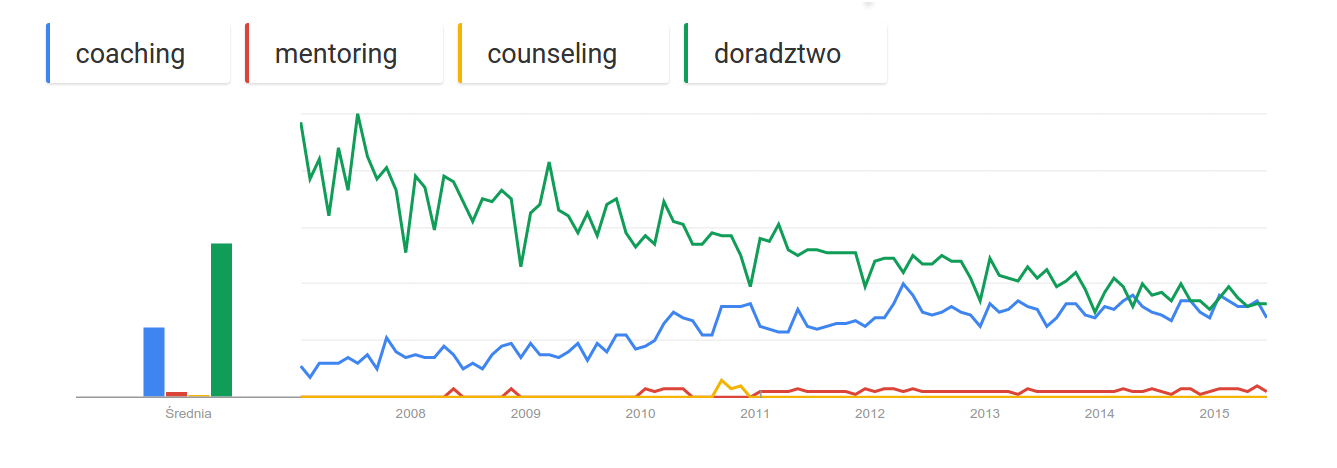
\includegraphics[width=17cm]{img/popularnosc}
  \caption{\TODO{opis}}
  \label{wykres}
\end{figure}

  \item Drugim szczególnie istotnym punktem w moim przeświadczeniu jest dyskrecja w sprawach dotyczących klienta.
      Cytując za Kodeksem Etycznym Izby Coachingu: "6.2 Jeśli dobro Klienta wchodzi w konflikt z lojalnością zawodową, Coach pracuje przede wszystkim dla dobra Klienta i postępuje zgodnie z uzgodnionym kontraktem.". Widocznym wnioskiem z tego punktu jest jak niezwykle ważne staje się czytelne ustalanie kontraktu pomiędzy coachem a klientem. Szczególna uwaga powinna mieć miejsce jeśli w proces zaangażowany jest również zewnętrzny zleceniodawca.
\end{itemize}

\subsection{Grupa docelowa procesu coachignowego}

\begin{itemize}
  \item im bardziej samodzielnym tym lepiej, ale przynajmniej w obszarze celów procesu
  \item osobom o wysokiej motywacji
  \item znajdującym się w nowej dla nich sytuacji (którym prawdopodobnie towarzyszy wysoka motywacja pozytywna) lub
       ulegających wypaleniu lub frustracji (wysoka motywacja negatywna). W drugim przypadku należy również rozważyć
       mentoring/szkolenia (np. frustracja wynika z braków wiedzy i przez to nie są osiągane efekty) lub consuelling \TODO{pisownia?}.
  \item dla osób stojących przed dylematem i aktywnie szukających jego rozwiązania
\end{itemize}

Tak jak zostało to podkreślone w poprzedniej sekcji - bardzo istotnym aspektem pracy coacha jest wiedza o tym, kiedy klient powinien
zostac skierowany do innego specjalisty. Przy pomocy tabeli \ref{table:kategorie} można zidentyfikować następujące przypadki:
\begin{itemize}
\item[--] W przypadku osoby potrzebującej wiedzy i gotowych rozwiązań - mentoring lub szkolenia.
\item[--] W przypadku osoby o niskiej motywacji / wypaleniu - consuelling.
\item[--] W przypadku osób stojących przed decyzją, ale nie dylematem - tzn. potrzebujących wiedzy i oceny sytuacji - pomoc konsultant.
\item[--] W przypadku osób w stanach depresyjnych, nie widzących możliwych rozwiązań i niskiej motywacji do wprowadzania zmian w swoim życiu - terapia.
\end{itemize}

\chapter{Zakończenie}

% Jak moge wykorzystac umiejetnosci i doswiadczenia nabyte w trakcie studiow i kontynuowac swoj rozwoj w roli coacha?
% Jakie dzialania zamierzam podjac, kto bedzie stanowic moja docelowa nisze?
% (z jakimi klientami i w jakich kontekstach mam zamiar pracowac?)
% Jaki zakres specjalizacji chcę rozwijac? Jakie dzialania praktyczne i kroki dalszego rozwoju (obszary doskonalenia) zamierzam podjac?

Autor pracy zamierza kontynuować swój rozwój osobisty i wykorzystać zdobyte w trakcie trwania studiów umiejętności na polu zawodowym.
W obecnym momencie nie zamierza, ani nie planuje w najbliższej przyszłości pracować jako coach, ponieważ prowadzi spółkę związaną z działalnością
zupełnie innego rodzaju. Rozwój osobisty traktuję jako pasję i na tym polu widzi swój potencjał do rozwoju, a w dalekiej przyszłości
chciałby realizować się w tej pasji pomagając innym.

Mając to na uwadze autor chciałby pielęgnować zdobyte umiejętności poprzez aktywne wykorzystywanie ich do autocoachingu i w życiu zawodowym.
W swojej dalekiej przyszłości chciałby pracować jako coach lub mentor dla osób lub zespołów realizujących projekty obarczone dużym ryzykiem.
Dopuszcza więc również możliwość pogłębienia swoich umiejętności w obszarze mentoringu lub szkoleń w niedługiej przyszłości.
Jako pierwszy cel na drodze realizacji tej wizji autor planuje udział w imprezach w obszarze nowych technologii
w charakterze coacha lub mentora - w perspektywie kilku kolejnych lat. Na tego typu wydarzeniach interdyscyplinarne zespoły mają za zadanie
w okresie kilku dni wymyślać innowacyjne rozwiązania wraz z pomysłem na ich komercjalizację.

Dodatkowo autor sam planuje rozpocząć pewien czas po zakończeniu studiów kolejny proces coachingowy - tym razem w charakterze osoby coachowanej.

\begin{thebibliography}{99}
\addcontentsline{toc}{chapter}{Bibliografia}

\bibitem{deficf} \textit{Definicja ICF}, \url{http://icf.org.pl/pl150,czym-jest-coaching-a-czym-nie-jest.html} (dostęp 06.2015)
\bibitem{kodeksicf} \textit{Kodeks etyczny ICF}, \url{ http://icf.org.pl/pl98,kodeks-etyczny-icf.html } (dostęp 06.2015)
\end{thebibliography}


\end{document}
